
The best way to understand how containers and iterators work is to experience them first-hand by creating your own. To avoid implementing something that already exists in the standard library, we will consider something different – more precisely, a circular buffer. This is a container that, when full, overwrites existing elements. We can think of different ways such a container could work; therefore, it’s important that we first define the requirements for it. These are as follows:

\begin{itemize}
\item
The container should have a fixed capacity that is known at compile-time. Therefore, there would be no runtime memory management.

\item
The capacity is the number of elements the container can store, and the size is the number of elements it actually contains. When the size equals the capacity, we say the container is full.

\item
When the container is full, adding a new element will overwrite the oldest element in the container.

\item
Adding new elements is always done at the end; removing existing elements is always done at the beginning (the oldest element in the container).

\item
There should be random access to the elements of the container, both with the subscript operator and with iterators.
\end{itemize}

Based on these requirements, we can think of the following implementation details:

\begin{itemize}
\item
The elements could be stored in an array. For convenience, this could be the std::array class.

\item
We need two variables, which we call head and tail, to store the index of the first and last elements of the container. This is needed because due to the circular nature of the container, the beginning

\item
A third variable will store the number of elements in the container. This is useful because otherwise, we would not be able to differentiate whether the container is empty or has one element only from the values of the head and tail indexes.

\begin{tcolorbox}[breakable,enhanced jigsaw,colback=blue!5!white,colframe=blue!75!black,title={Important Note}]
The implementation shown here is provided for teaching purposes only and is not intended as a production-ready solution. The experienced reader will find different aspects of the implementation that could be optimized. However, the purpose here is to learn how to write a container and not how to optimize the implementation.
\end{tcolorbox}

\end{itemize}

The following diagram shows a visual representation of such a circular buffer, with a capacity of eight elements with different states:

\begin{center}
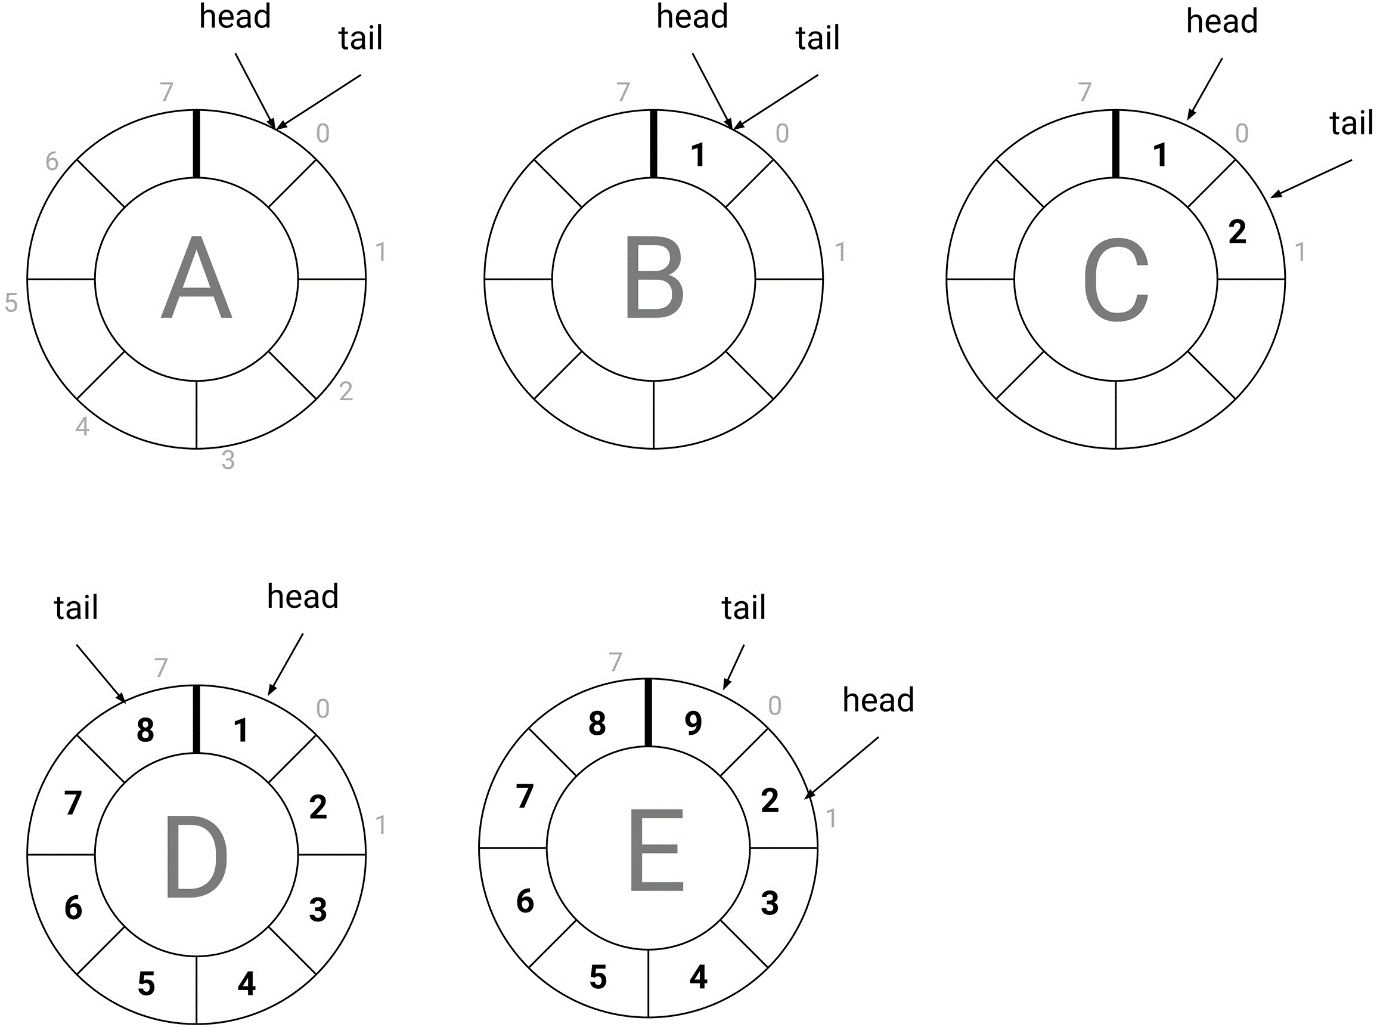
\includegraphics[width=0.8\textwidth]{content/3/chapter8/images/2.png}\\
Figure 8.2
\end{center}

What we can see in this diagram is the following:

\begin{itemize}
\item
Figure A: This is an empty buffer. The capacity is 8, the size is 0, and the head and tail both point to index 0.

\item
Figure B: This buffer contains one element. The capacity is still 8, the size is 1, and the head and tail both still point to index 0.

\item
Figure C: This buffer contains two elements. The size is 2, the head contains index 0, and the tail contains index 1.

\item
Figure D: This buffer is full. The size is 8, which is equal to the capacity, and the head contains index 0 and the tail contains index 7.

\item
Figure E: This buffer is still full, but an additional element has been added, triggering the overwriting of the oldest element in the buffer. The size is 8, the head contains index 1, and the tail contains index 0.
\end{itemize}

Now that we have looked at the semantics of the circular buffer, we can start writing the implementation. We will begin with the container class.

\subsubsubsection{8.2.1\hspace{0.2cm}Implementing a circular buffer container}

The code for the container class would be too long to be put in a single listing, so we’ll break it up into multiple snippets. The first is as follows:

\begin{lstlisting}[style=styleCXX]
template <typename T, std::size_t N>
	requires(N > 0)
class circular_buffer_iterator;

template <typename T, std::size_t N>
	requires(N > 0)
class circular_buffer
{
	// ...
};
\end{lstlisting}

There are two things here: the forward declaration of a class template called circular\_buffer\_iterator, and a class template called circular\_buffer. Both have the same template arguments, a type template parameter T, representing the type of the elements, and a non-type template parameter, representing the capacity of the buffer. A constraint is used to ensure that the provided value for capacity is always positive. If you are not using C++20, you can replace the constraint with a static\_assert statement or enable\_if to enforce the same restriction. The following snippets are all part of the circular\_buffer class.

First, we have a series of member type definitions that provide aliases to different types that are relevant to the circular\_buffer class template. These will be used in the implementation of the class. They are shown next:

\begin{lstlisting}[style=styleCXX]
	public:
	using value_type = T;
	using size_type = std::size_t;
	using difference_type = std::ptrdiff_t;
	using reference = value_type&;
	using const_reference = value_type const&;
	using pointer = value_type*;
	using const_pointer = value_type const*;
	using iterator = circular_buffer_iterator<T, N>;
	using const_iterator =
	circular_buffer_iterator<T const, N>;
\end{lstlisting}

Second, we have the data members that store the buffer state. The actual elements are stored in a std::array object. The head, tail, and size are all stored in a variable of the size\_type data type. These members are all private:

\begin{lstlisting}[style=styleCXX]
private:
	std::array<value_type, N> data_;
	size_type head_ = 0;
	size_type tail_ = 0;
	size_type size_ = 0;
\end{lstlisting}

Third, we have the member functions that implement the functionality described earlier. All the following members are public. The first to list here are the constructors:

\begin{lstlisting}[style=styleCXX]
constexpr circular_buffer() = default;
constexpr circular_buffer(value_type const (&values)[N]) :
	size_(N), tail_(N-1)
{
	std::copy(std::begin(values), std::end(values),
	data_.begin());
}
constexpr circular_buffer(const_reference v):
	size_(N), tail_(N-1)
{
	std::fill(data_.begin(), data_.end(), v);
}
\end{lstlisting}

There are three constructors defined here (although we can think of additional ones). These are the default constructor (which is also defaulted) that initializes an empty buffer, a constructor from a C-like array of size N, which initializes a full buffer by copying the array elements, and, finally, a constructor that takes a single value and initializes a full buffer by copying that value into each element of the buffer. These constructors allow us to create circular buffers in any of the following ways:

\begin{lstlisting}[style=styleCXX]
circular_buffer<int, 1> b1; // {}
circular_buffer<int, 3> b2({ 1, 2, 3 }); // {1, 2, 3}
circular_buffer<int, 3> b3(42); // {42, 42, 42}
\end{lstlisting}

Next, we define several member functions that describe the state of the circular buffer:

\begin{lstlisting}[style=styleCXX]
constexpr size_type size() const noexcept
{ return size_; }

constexpr size_type capacity() const noexcept
{ return N; }

constexpr bool empty() const noexcept
{ return size_ == 0; }

constexpr bool full() const noexcept
{ return size_ == N; }

constexpr void clear() noexcept
{ size_ = 0; head_ = 0; tail_ = 0; };
\end{lstlisting}

The size function returns the number of elements in the buffer, the capacity function the number of elements that the buffer can hold, the empty function to check whether the buffer has no elements (the same as size() == 0), and the full function to check whether the buffer is full (the same as size() == N). There is also a function called clear that puts the circular buffer in the empty state. Beware that this function doesn't destroy any element (does not release memory or call destructors) but only resets the values defining the state of the buffer.

We need to access the elements of the buffer; therefore, the following functions are defined for this purpose:

\begin{lstlisting}[style=styleCXX]
constexpr reference operator[](size_type const pos)
{
	return data_[(head_ + pos) % N];
}

constexpr const_reference operator[](size_type const pos) const
{
	return data_[(head_ + pos) % N];
}

constexpr reference at(size_type const pos)
{
	if (pos < size_)
		return data_[(head_ + pos) % N];
		
	throw std::out_of_range("Index is out of range");
}

constexpr const_reference at(size_type const pos) const
{
	if (pos < size_)
		return data_[(head_ + pos) % N];
		
	throw std::out_of_range("Index is out of range");
}

constexpr reference front()
{
	if (size_ > 0) return data_[head_];
	throw std::logic_error("Buffer is empty");
}

constexpr const_reference front() const
{
	if (size_ > 0) return data_[head_];
	throw std::logic_error("Buffer is empty");
}

constexpr reference back()
{
	if (size_ > 0) return data_[tail_];
	throw std::logic_error("Buffer is empty");
}

constexpr const_reference back() const
{
	if (size_ > 0) return data_[tail_];
	throw std::logic_error("Buffer is empty");
}
\end{lstlisting}

Each of these members has a const overload that is called for constant instances of the buffer. The constant member returns a constant reference; the non-const member returns a normal reference. These methods are as follows:

\begin{itemize}
\item
The subscript operator that returns a reference to the element specified by its index, without checking the value of the index

\item
The at method that works similarly to the subscript operator, except that it checks that the index is smaller than the size and, if not, throws an exception

\item
The front method that returns a reference to the first element; if the buffer is empty, it throws an exception

\item
The back method that returns a reference to the last element; if the buffer is empty, it throws an exception
\end{itemize}

We have members to access the elements, but we need members for adding and removing elements to/from the buffer. Adding new elements always happens at the end, so we’ll call this push\_back. Removing existing elements always happens at the beginning (the oldest element), so we’ll call this pop\_front. Let’s look first at the former:

\begin{lstlisting}[style=styleCXX]
constexpr void push_back(T const& value)
{
	if (empty())
	{
		data_[tail_] = value;
		size_++;
	}
	else if (!full())
	{
		data_[++tail_] = value;
		size_++;
	}
	else
	{
		head_ = (head_ + 1) % N;
		tail_ = (tail_ + 1) % N;
		data_[tail_] = value;
	}
}
\end{lstlisting}

This works based on the defined requirements and the visual representations from Figure 8.2:

\begin{itemize}
\item
If the buffer is empty, copy the value to the element pointed by the tail\_ index and increment the size.

\item
If the buffer is neither empty nor full, do the same but also increment the value of the tail\_ index.

\item
If the buffer is full, increment both the head\_ and the tail\_ and then copy the value to the element pointed by the tail\_ index.
\end{itemize}

This function copies the value argument to a buffer element. However, this could be optimized for temporaries or objects that are no longer needed after pushing to the buffer. Therefore, an overload that takes an rvalue reference is provided. This moves the value to the buffer, avoiding an unnecessary copy. This overload is shown in the following snippet:

\begin{lstlisting}[style=styleCXX]
constexpr void push_back(T&& value)
{
	if (empty())
	{
		data_[tail_] = value;
		size_++;
	}
	else if (!full())
	{
		data_[++tail_] = std::move(value);
		size_++;
	}
	else
	{
	head_ = (head_ + 1) % N;
	tail_ = (tail_ + 1) % N;
	data_[tail_] = std::move(value);
	}
}
\end{lstlisting}

A similar approach is used for implementing the pop\_back function to remove elements from the buffer. Here is the implementation:

\begin{lstlisting}[style=styleCXX]
constexpr T pop_front()
{
	if (empty()) throw std::logic_error("Buffer is empty");
	
	size_type index = head_;
	
	head_ = (head_ + 1) % N;
	size_--;
	
	return data_[index];
}
\end{lstlisting}

This function throws an exception if the buffer is empty. Otherwise, it increments the value of the head\_ index and returns the value of the element from the previous position of the head\_. This is described visually in the following diagram:

\begin{center}
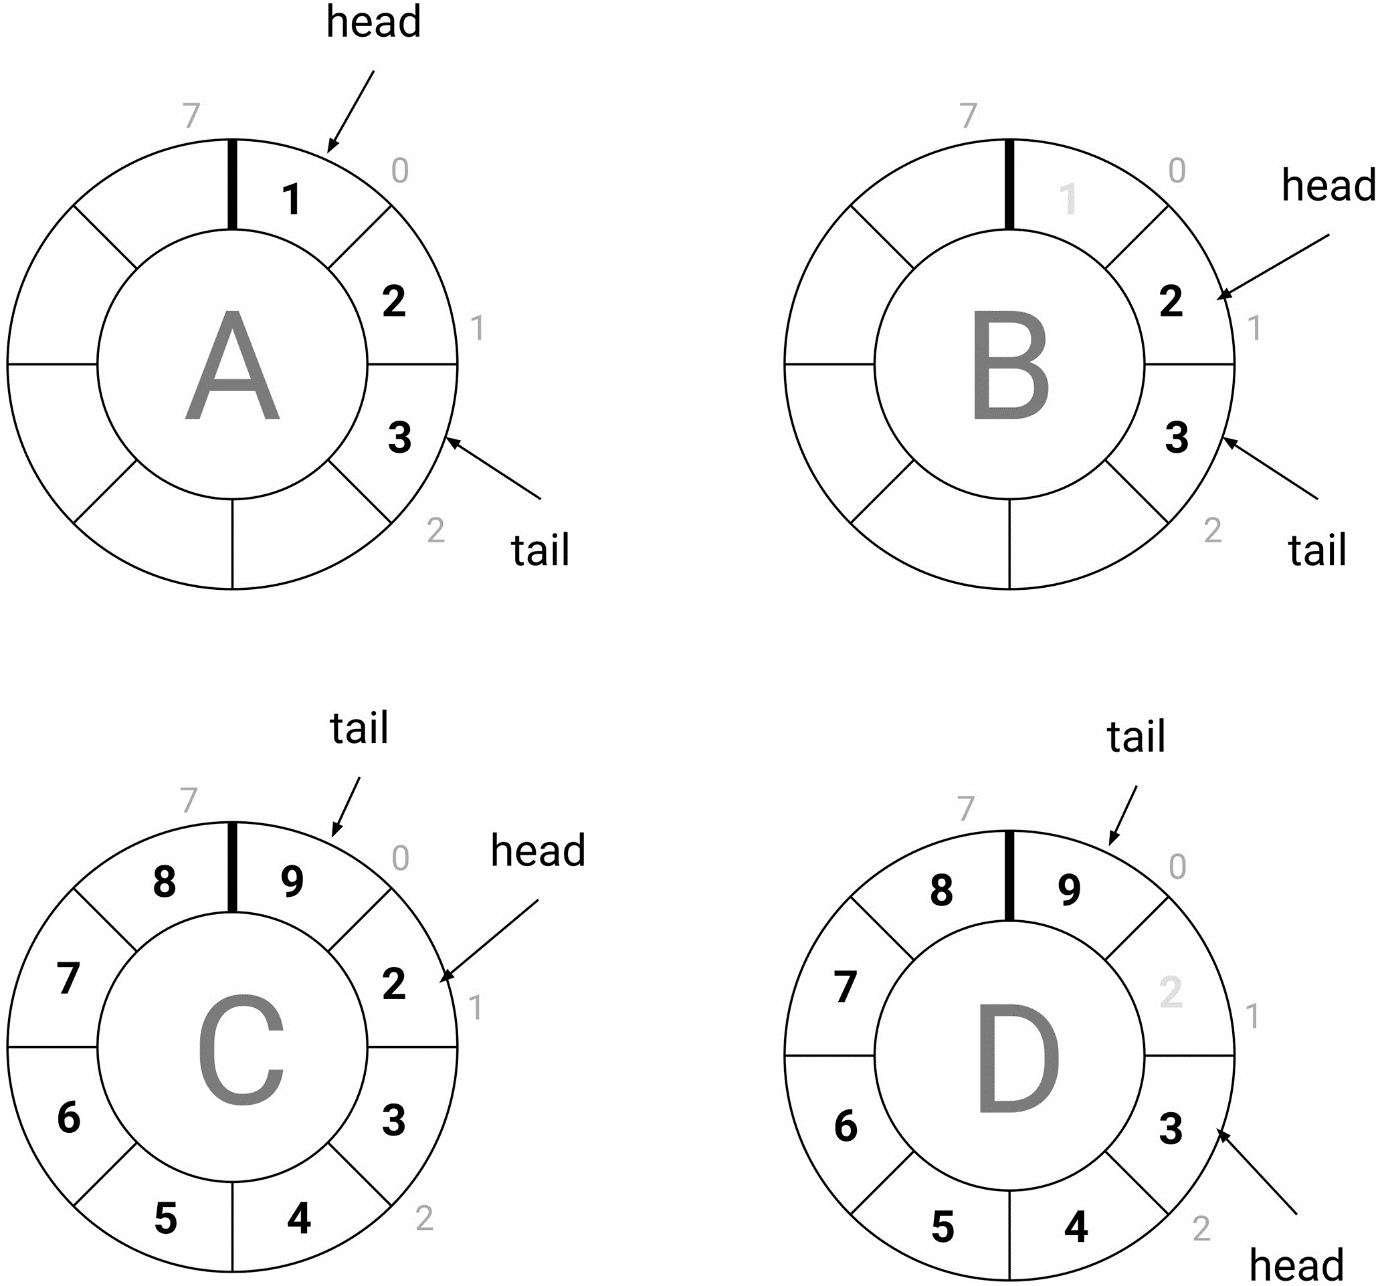
\includegraphics[width=0.7\textwidth]{content/3/chapter8/images/3.png}\\
Figure 8.3
\end{center}

What we can see here is the following:

\begin{itemize}
\item
Figure A: The buffer has 3 elements (1, 2, and 3), head is at index 0, and tail is at index 2.

\item
Figure B: An element has been removed from the front, which was index 0. Therefore, head is now index 1 and tail is still index 2. The buffer now has two elements.

\item
Figure C: The buffer has eight elements, which is its maximum capacity, and an element has been overwritten. The head is at index 1 and the tail is at index 0.

\item
Figure D: An element has been removed from the front, which was index 1. The head is now at index 2 and the tail is still at index 0. The buffer now has seven elements.
\end{itemize}

An example of using both the push\_back and the pop\_front member functions is shown in the next snippet:

\begin{lstlisting}[style=styleCXX]
circular_buffer<int, 4> b({ 1, 2, 3, 4 });
assert(b.size() == 4);

b.push_back(5);
b.push_back(6);
b.pop_front();

assert(b.size() == 3);
assert(b[0] == 4);
assert(b[1] == 5);
assert(b[2] == 6);
\end{lstlisting}

Finally, we have the member functions begin and end that return iterators to the first and one-past-the-last elements of the buffer. Here is their implementation:

\begin{lstlisting}[style=styleCXX]
iterator begin()
{
	return iterator(*this, 0);
}

iterator end()
{
	return iterator(*this, size_);
}

const_iterator begin() const
{
	return const_iterator(*this, 0);
}

const_iterator end() const
{
	return const_iterator(*this, size_);
}
\end{lstlisting}

To understand these, we need to see how the iterator class is actually implemented. We will explore this in the next section.

\subsubsubsection{8.2.2\hspace{0.2cm}Implementing an iterator type for the circular buffer container}

We declared the iterator class template at the beginning of the previous section when we started with the circular\_buffer container. However, we need to define its implementation too. Yet, there is one more thing we must do: in order for the iterator class to be able to access the private members of the container it needs to be declared as a friend. This is done as follows:

\begin{lstlisting}[style=styleCXX]
private:
	friend circular_buffer_iterator<T, N>;
\end{lstlisting}

Let’s look now at the circular\_buffer\_iterator class, which actually has similarities with the container class. This includes the template parameters, the constraints, and the set of member types (some of them being common to those in circular\_buffer). Here is a snippet of the class:

\begin{lstlisting}[style=styleCXX]
template <typename T, std::size_t N>
requires(N > 0)
class circular_buffer_iterator
{
public:
	using self_type = circular_buffer_iterator<T, N>;
	using value_type = T;
	using reference = value_type&;
	using const_reference = value_type const &;
	using pointer = value_type*;
	using const_pointer = value_type const*;
	using iterator_category =
		std::random_access_iterator_tag;
	using size_type = std::size_t;
	using difference_type = std::ptrdiff_t;
public:
	/* definitions */
	
private:
	std::reference_wrapper<circular_buffer<T, N>> buffer_;
	size_type index_ = 0;
};
\end{lstlisting}

The circular\_buffer\_iterator class has a reference to a circular buffer and an index to the element in the buffer that it points to. The reference to circular\_buffer<T, N> is wrapped inside a std::reference\_wrapper object. The reason for this will be unveiled shortly. Such an iterator can be explicitly created by providing these two arguments. Therefore, the only constructor looks as follows:

\begin{lstlisting}[style=styleCXX]
explicit circular_buffer_iterator(
	circular_buffer<T, N>& buffer,
	size_type const index):
	buffer_(buffer), index_(index)
{ }
\end{lstlisting}

If we now look back at the definitions of the begin and end member functions of circular\_buffer, we can see that the first argument was *this, and the second was 0 for the begin iterator and size\_ for the end iterator. The second value is the offset from the head of the element pointed by the iterator. Therefore, 0 is the first element, and size\_ is the one-past-the-last element in the buffer.

We have decided that we need random access to the elements of the buffer; therefore, the iterator category is random-access. The member type iterator\_category is an alias for std::random\_access\_iterator\_tag. This implies that we need to provide all the operations supported for such an iterator. In the previous section of this chapter, we discussed the iterator categories and the required operations for each category. We will implement all the required ones next.

We start with the requirements for an input iterator, which are as follows:

\begin{lstlisting}[style=styleCXX]
self_type& operator++()
{
	if(index_ >= buffer_.get().size())
		throw std::out_of_range("Iterator cannot be
								incremented past the end of the range");
								
	index_++;
	return *this;
}

self_type operator++(int)
{
	self_type temp = *this;
	++*this;
	return temp;
}

bool operator==(self_type const& other) const
{
	return compatible(other) && index_ == other.index_;
}

bool operator!=(self_type const& other) const
{
	return !(*this == other);
}

const_reference operator*() const
{
	if (buffer_.get().empty() || !in_bounds())
		throw std::logic_error("Cannot dereferentiate the
	iterator");
	return buffer_.get().data_[
		(buffer_.get().head_ + index_) %
		 buffer_.get().capacity()];
}

const_reference operator->() const
{
	if (buffer_.get().empty() || !in_bounds())
		throw std::logic_error("Cannot dereferentiate the
								iterator");
								
	return buffer_.get().data_[
		(buffer_.get().head_ + index_) %
		 buffer_.get().capacity()];
}
\end{lstlisting}

We have implemented here incrementing (both pre- and post-fix), checking for equality/ inequality, and dereferencing. The * and -> operators throw an exception if the element cannot be dereferenced. The cases when this happens are when the buffer is empty, or the index is not within bounds (between head\_ and tail\_). We used two helper functions (both private), called compatible and is\_bounds. These are shown next:

\begin{lstlisting}[style=styleCXX]
bool compatible(self_type const& other) const
{
	return buffer_.get().data_.data() ==
		   other.buffer_.get().data_.data();
}

bool in_bounds() const
{
	return
		!buffer_.get().empty() &&
		(buffer_.get().head_ + index_) %
		 buffer_.get().capacity() <= buffer_.get().tail_;
}
\end{lstlisting}

A forward iterator is an input iterator that is also an output iterator. The requirements for output iterators will be discussed toward the end of this section. Those for the input iterators we have seen previously. Apart from those, forward iterators can be used in multi-pass algorithms, which is possible because performing an operation on a dereferenceable forward iterator does not make its iterator value non-dereferenceable. That means if a and b are two forward iterators and they are equal, then either they are non-dereferenceable, otherwise, their iterator values, *a and *b, refer to the same object. The opposite is also true, meaning that if *a and *b are equal, then a and b are also equal. This is true for our implementation.

The other requirement for forward iterators is that they are swappable. That means if a and b are two forward iterators, then swap(a, b) should be a valid operation. This leads us back to using a std::reference\_wrapper object to hold a reference to a circular\_buffer<T, N>. References are not swappable, which would have made circular\_buffer\_iterator not swappable either. However, std::reference\_wrapper is swappable, and that also makes our iterator type swappable. That can be verified with a static\_assert statement, such as the following:

\begin{lstlisting}[style=styleCXX]
static_assert(
	std::is_swappable_v<circular_buffer_iterator<int, 10>>);
\end{lstlisting}

\begin{tcolorbox}[breakable,enhanced jigsaw,colback=blue!5!white,colframe=blue!75!black,title={Important Note}]
An alternative to using std::reference\_wrapper is to use a raw pointer to a circular\_buffer class, since pointers can be assigned values and are, therefore swappable. It is a matter of style and personal choice which one to use. In this example, I preferred the solution that avoided the raw pointer.
\end{tcolorbox}

For fulfilling the requirements for the bidirectional iterator category, we need to support decrementing. In the next snippet, you can see the implementation of both pre- and post-fix decrement operators:

\begin{lstlisting}[style=styleCXX]
self_type& operator--()
{
	if(index_ <= 0)
		throw std::out_of_range("Iterator cannot be
			decremented before the beginning of the range");
			
	index_--;
	return *this;
}

self_type operator--(int)
{
	self_type temp = *this;
	--*this;
	return temp;
}
\end{lstlisting}

Finally, we have the requirements of the random-access iterators. The first requirements to implement are arithmetic (+ and -) and compound (+= and -=) operations. These are shown next:

\begin{lstlisting}[style=styleCXX]
self_type operator+(difference_type offset) const
{
	self_type temp = *this;
	return temp += offset;
}

self_type operator-(difference_type offset) const
{
	self_type temp = *this;
	return temp -= offset;
}

difference_type operator-(self_type const& other) const
{
	return index_ - other.index_;
}

self_type& operator +=(difference_type const offset)
{
	difference_type next =
		(index_ + next) % buffer_.get().capacity();
	if (next >= buffer_.get().size())
		throw std::out_of_range("Iterator cannot be
								 incremented past the bounds of the range");
								 
	index_ = next;
	return *this;
}

self_type& operator -=(difference_type const offset)
{
	return *this += -offset;
}
\end{lstlisting}

Random-access iterators must support inequality comparison with other operations. That means, we need to overload the <, <=, >, and >= operators. However, the <=, >, and >= operators can be implemented based on the < operator. Therefore, their definition can be as follows:

\begin{lstlisting}[style=styleCXX]
bool operator<(self_type const& other) const
{
	return index_ < other.index_;
}

bool operator>(self_type const& other) const
{
	return other < *this;
}

bool operator<=(self_type const& other) const
{
	return !(other < *this);
}

bool operator>=(self_type const& other) const
{
	return !(*this < other);
}
\end{lstlisting}

Last, but not least, we need to provide access to elements with the subscript operator ([]). A possible implementation is the following: 

\begin{lstlisting}[style=styleCXX]
value_type& operator[](difference_type const offset)
{
	return *((*this + offset));
}

value_type const & operator[](difference_type const offset)
const
{
	return *((*this + offset));
}
\end{lstlisting}

With this, we have completed the implementation of the iterator type for the circular buffer. If you had trouble following the multitude of code snippets for these two classes, you can find the complete implementation in the GitHub repository for the book. A simple example for using the iterator type is shown next:

\begin{lstlisting}[style=styleCXX]
circular_buffer<int, 3> b({1, 2, 3});
std::vector<int> v;
for (auto it = b.begin(); it != b.end(); ++it)
{
	v.push_back(*it);
}
\end{lstlisting}

This code can be actually simplified with range-based for loops. In this case, we don’t use iterators directly, but the compiler-generated code does. Therefore, the following snippet is equivalent to the previous one:

\begin{lstlisting}[style=styleCXX]
circular_buffer<int, 3> b({ 1, 2, 3 });
std::vector<int> v;
for (auto const e : b)
{
	v.push_back(e);
}
\end{lstlisting}

However, the implementation provided here for circular\_buffer\_iterator does not allow the following piece of code to compile:

\begin{lstlisting}[style=styleCXX]
circular_buffer<int, 3> b({ 1,2,3 });
*b.begin() = 0;

assert(b.front() == 0);
\end{lstlisting}

This requires that we are able to write elements through iterators. However, our implementation doesn’t meet the requirements for the output iterator category. This requires that expressions such as *it = v, or *it++ = v are valid. To do so, we need to provide non-const overloads of the * and -> operators that return non-const reference types. This can be done as follows:

\begin{lstlisting}[style=styleCXX]
reference operator*()
{
	if (buffer_.get().empty() || !in_bounds())
		throw std::logic_error("Cannot dereferentiate the
								iterator");
	
	return buffer_.get().data_[
		(buffer_.get().head_ + index_) %
		 buffer_.get().capacity()];
}

reference operator->()
{
	if (buffer_.get().empty() || !in_bounds())
		throw std::logic_error("Cannot dereferentiate the
								iterator");
								
	return buffer_.get().data_[
		(buffer_.get().head_ + index_) %
		 buffer_.get().capacity()];
}
\end{lstlisting}

More examples for using the circular\_buffer class with and without iterators can be found in the GitHub repository. Next, we will focus our attention on implementing a general-purpose algorithm that works for any range, including the circular\_buffer container we defined here.






















